\begin{evenBlock}{Cone Weave Dribbling}


\begin{minipage}[t]{\linewidth}
    \centering
    
    \begin{minipage}{.3\linewidth} % Left column and width
        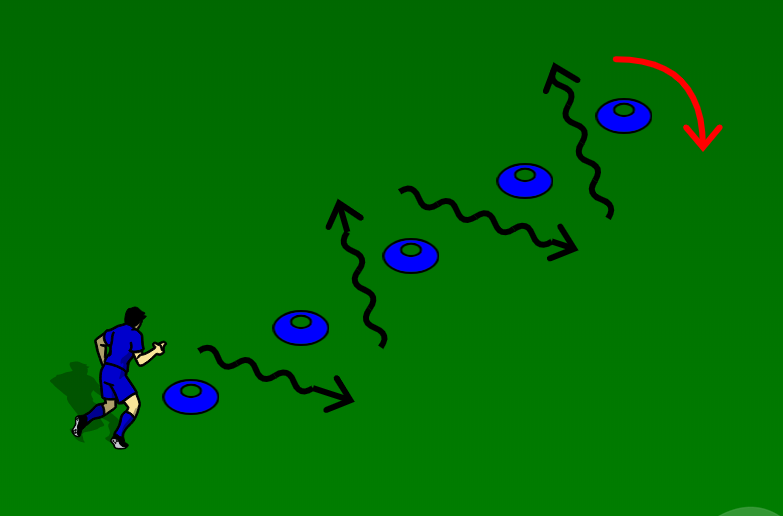
\includegraphics[width=\textwidth]{../img/Trimmed/cone_dribbling}
    \end{minipage}
    \hspace{0.05\linewidth}
    \begin{minipage}{.6\linewidth} % Left column and width
        \textbf{Drill Description:}
        Dribble around 6 cones about 1 yard apart, using only the inside portion of the foot to make cuts.  Ends are different color, orange inside cut, green outside cut.  Players should focus on using 3 touches to make the turn around the end cones.

        \vspace{3pt}
        
        Advanced - use only the outside of the foot or alternate inside foot one direction, outside foot when traveling the other direction.
        %\end{enumerate}

        \vspace{10pt}
        
        \textbf{Coaching Points:}
        \begin{itemize}
        \setlength{\itemsep}{0pt}
        \setlength{\parskip}{0pt}
        \setlength{\parsep}{0pt}
        \item Go slow at first and work up speed as control increases.
        \item Control should be the focus of this drill.  As control increases, increase speed.
        \item Players should always be on their toes, no standing flat footed.
        \item Its better to have 3-5 small controlled touches around the last cone than 3 large out of control touches.
        \end{itemize}

    \end{minipage}
\end{minipage}

\end{evenBlock}